\chapter[Construire un corpus historique]{Construire un Corpus historique pour la vision artificielle}

\lettrine{L}{ors de} notre stage, l'objectif à atteindre était de contribuer à la préparation d'une campagne collaborative de constitution d'un jeu de données annoté de documents historiques. L'objectif est de créer un corpus de référence pour l'entraînement de modèles d'extraction automatique de classes visuelles (illustration, photographies, zones de texte, enluminures, etc.). Le stage consistait à définir le cadre méthodologique et technique du dispositif à l'aide de la préparation d'un jeu de données de test.

\section{La nature documentaire du Corpus}

GenHisDoc (\textit{Generalistic Historical Document Dataset}) et ses modèles associés est le jeu de données que nous avons créer lors de ce stage. Les trois questions au coeur de sa création sont : l'harmonisation de corpus hétérogènes pour une réutilisation, l'enrichissement du corpus par la pratique historienne en réutilisant les données produites par Aikon, l'impact que produit une ontologie documentaire sur la performance algorithmique.


\subsection{La réutilisation des jeux de données existants}

Le volume de donnée de qualité pour entraîné un modèle spécialisé performant mieux que ce qui existe déjà demande une autre technique que la création de données \textit{ex nihilo}. De plus, l'un des buts du stage était d'entraîner un modèle aussi efficace sur les livres imprimés que sur les manuscrits. Il existe déjà des corpus spécialisés ouverts et publié sur licence libre permettant une réutilisation et une modification des données. Pour ces raisons de droit, nous avons réutilisé aucune données venant de compétitions comme ICDAR car la plupart sont produit par PRImA Research, un groupe de recherche de l'université de Stalford Manchester dont la plupart des datasets sont sous-droit.

La plupart des jeux de données que nous avons sélectionné pour une réutilisation étaient sous une licence \textit{Creative Common}. Pensez comme un compromis flexible au \og tous droits réservés \fg, les licences\textit{ Creative Commons} offrent un cadre juridique standardisé pour autoriser la libre réutilisation des ressources numériques. En articulant différentes contraintes modulables, de la simple mention de paternité à la restriction des usages commerciaux, ce système simplifie l'ouverture des données patrimoniales et garantit aux chercheurs une sécurité juridique essentielle lors du partage et de la réexploitation des corpus. Dans le domaine de la vision, la plupart des datasets récents utilisent l'attribution 4.0 International (CC BY 4.0) permettant de partager et de réutiliser sur ces ressources à condition de créditer l'auteur original. Dans le cadre de GenHisDoc le crédit ce fait de trois manières : 

\begin{itemize}
    \item Premièrement, dans le README de la publication finale de GenHisDoc, tous les datasets réutilisés sont cités, ainsi que leurs auteurs connus, et les datapapers ayant été publiés pour ces jeux de données.

    \item Deuxièmement, bien que la version du finale du jeu de données mélange ensemble toutes les images et toutes les annotations en deux grands dossiers \textit{Images} et \textit{Annotations}, le script de \og réunification \og des données produit également un lien entre la source de publication de l'image et son nom dans le dataset final disponible dans un format csv. 

    \item Troisièmement, dans le cadre de la réutilisation des données d'Aikon nous nommons les utilisateurs ayant uploadé, inférencé ou corrigé les données que nous avons téléchargé. 

\end{itemize}

Cependant, le potentiel de ces ressources est fréquemment freiné par une hétérogénéité technique et une spécialisation conceptuelle. La première partie de notre travail était d'identifier, agréger et comparer le plus de jeux de données éligible entre eux\footnote{Konstantina Nikolaidou, Mathias Seuret, Hamam Mokayed, Marcus Liwicki, \og A survey of historical document image datasets \fg, dans \textit{International Journal on Document Analysis and Recognition (IJDAR)}, pp.305-338, n°25, vol 4, 2022}. Cette démarche de réutilisation s'est heurtée à deux défis majeurs. Le premier est d'ordre technique avec la diversité des formats d'annotation (segmentation sémantique par pixels, différents types de coordonnés sur l'image pour la boîte englobante) empêche tout entraînement conjoint. Le second étant d'ordre intellectuel où chaque projet de recherche définit son ontologie et ses propres classes d'annotation en fonction de ses problématiques scientifiques, rendant certains jeux de données incompatible entre eux. 

\begin{description}
\item[S-VED :]

\subitem \textbf{Classes :} Illustration, Ornementation, Lettrine, Marque d'imprimeur

\subitem \textbf{Édition :} Issue du projet \textit{De Spherae} de la Max Planck Institute for the History of Science, le dataset S-VED propose un jeu de données constitués d'exemples tirés des 350 éditions du \textit{Tractatus de Spherae} de Johannes de Sacrobosco annotées et compilées ensembles\footnote{Büttner J, Martinetz J, El-Hajj H, Valleriani M, \og CorDeep and the Sacrobosco Dataset: Detection of Visual Elements in Historical Documents \fg, dans \textit{Journal of Imaging}, n°8, volume 10,  pp.285 , 2022,  DOI : \href{10.3390/jimaging8100285}{10.3390/jimaging8100285}}. S-VED  est un projet qui privilégie la simplicité et la facilité d'usage de ses annotations et de son format d'ontologie. S-VED existe en deux versions, une sous-droit et une purgée de ses documents problématiques. Nous avons donc utilisé la deuxième version. Parmi les principales corrections que nous avons du faire à S-VED, la première était la suppression de la classe des marques d'imprimeurs qui ne fait pas sens au sein d'une ontologie généraliste. 

%%%%%%%%%%%%%%%%%%%%%%%%

\item[IlluHisDoc :] 

\subitem \textbf{Classes :} Photographie, Illustration, Dessins, Diagramme scientifiques historiques

\subitem \textbf{Édition :} Issue du projet docExtractor de Tom Monier et Mathieu Aubry\footnote{Tom Monnier, Mathieu Aubry, « docExtractor : An off-the-shelf historical document element extrac-tion »,dans2020 17th International Conference on Frontiers in Handwriting Recognition(ICFHR), pp. 91-96,2020, DOI : 10.1109/ICFHR2020.2020.00027}. D'un point de vue technique, le jeu de données proposait une segmentation sémantique au niveau du pixel, que nous avons transformer en boîtes englobantes au format YOLO\footnote{Jules Musquin avec 4 classes : \href{https://github.com/Anarchiviste/GenHisDoc\_Lab/blob/main/01\_code/reconciliation\_illuhisdoc.py}{scripte reconcialiation\_IlluHisDoc.py sur GenHisDoc\_Lab github}}. D'un point de vue éditorial, la classe très spécifique correspondant aux marques d'imprimeur (printer's marks) a été fusionnée avec notre classe générale \og Illustration \fg afin de maintenir l'approche généraliste de GenHisDoc.

%%%%%%%%%%%%%%%%%%%%%%%

\item[Horae LSv2 :] 

\subitem \textbf{Classes :} Lignes de texte, Lettrines, Ornementations, Zone de texte, Pages, Rubrication, Miniature. 

\subitem \textbf{Édition :} Horae est un jeu de données constitué principalement de livre d'heure. D'un point de vue technique, Horae est déjà pensé pour une compatibilité avec les modèles Yolo. D'un point de vue éditorial, nous avons supprimé toutes les classes liées au texte, regrouper toutes les classes liées aux lettrines, liées toutes les classes liées aux ornementations et liées toutes les classes liées aux illustrations. 

%%%%%%%%%%%%%%%%%%%%%%

\item[El Picpic Stamps :] 

\subitem \textbf{Classes :} Tampons, Signatures
\subitem \textbf{Édition :} C'est à la base un jeu de données publiées sur la plateforme Roboflow sous licence CC by 4.0 par l'utilisateur \textit{El PicPic}. Le jeu de données avait comme but de détecter les tampons et les signatures, nous avons donc supprimés toutes les annotations de signatures. D'un point de vue technique nous avons transformer des boîtes englobantes en coordonnés généraux au format Yolo.

\end{description}

Nous avons aussi travaillé sur l'intégration de documents et de jeux de données qui n'ont pas terminé dans le dataset final. Dans la volonté de produire un jeu de données généraliste capable de fonctionner autant sur un manuscrit médiévale que sur des sources imprimés, nous avons voulu trouver un moyen d'intégrer des sources de presses dans notre ontologie très simple. 

\subsection{Récupérer des données d'Aikon}


Outre l'exploitation de jeux de données publics indépendants, une part déterminante de la constitution de GenHisDoc repose sur la récupération directe de métadonnées produites au sein même de la plateforme AIkon. L'infrastructure d'annotation automatique et de partage des documents dans l'application se fait via le protocole IIIF. Au sein d'Aikon, quand un document récupéré entièrement sur l'application est nommé un \og témoin \fg  (\textit{witnesses}). 

L'utilisation du standard IIIF nous a permis de développer un outil en ligne de commande (CLI) nommé \textit{aikoncli} pour récupérer toutes les pages qui constituent un témoins ainsi que toutes les annotations qui y sont attachées et directement au format YOLO en fournissant le manifeste IIIF de l'instance d'AIkon\footnote{Jules Musquin, \href{https://github.com/Anarchiviste/aikoncli}{\textit{aikoncli} sur GitHub}}.

Les témoins récupérés 
\begin{description}
\item[VHS :] Ce projet interdisciplinaire étudie la circulation de l'illustration scientifique du Moyen Âge à l'ère moderne. Nous avons extrait les données issues de neuf témoins révisés par les chercheurs du projet, couvrant à la fois des imprimés (telle la \textit{Cyclopaedia} d'Ephraïm Chambers) et des manuscrits d'astronomie et de sciences conservés dans de grandes institutions européennes\footnote{Notamment les manuscrits BnF Latin 7416 et Latin 13955 ; ÖNB Cod. 44 et 187 ; Universiteitsbibliotheek Lat. Q. 9 et Voss. Lat. Q. 40 ; Biblioteca Ambrosiana T. 47 ; Sächsische Landesbibliothek Dc 183.}.

\item[EIDA :] Centré sur l'analyse critique des diagrammes astronomiques du VIII\textsuperscript{e} au XVIII\textsuperscript{e} siècle, le projet EIDA apporte une diversité culturelle et typologique indispensable à GenHisDoc. L'extraction a permis d'intégrer des corpus issus de traditions manuscrites non occidentales (sanskrite, turque ottomane, arabo-persane) comme les témoins BnF Sanscrit 964 et Supplément turc 242, ou le manuscrit Sprenger 1838 de la Staatsbibliothek de Berlin.
\end{description}

Une fois un témoin choisi comme étant intéressant à ajouter dans le jeu de données, nous avons fait le choix de ne pas trier les pages internes du document. Le but est de de préserver dans le jeu de données un ratio d'images représentant des pages vides, des pages de titre, des images sans annotations, des images des dos des livres, des images des pages d'information de la BnF insérés dans les pdf téléchargés depuis Gallica. Le but étant de réduire la détection d'élément indésirables en augmentant un peu le bruit dans les données. 

L'intégration de ces corpus d'AIkon représentent un apport précieux pour GenHisDoc, notamment pour la représentativité des schémas et des diagrammes scientifiques. Néanmoins, les modèles historiques d'AIkon fonctionnant sur une détection purement monoclasse (repérant un composant visuel sans qualification typologique), ces données ont donc été traduit par la classe \textit{Illustration} dans l'ontologie de GenHisDoc. 

\section{La nature technique du corpus}

Une fois les sources sélectionnées et l'ontologie décidée, la constitution de GenHisDoc s'est heurtée à la matérialité technique de la donnée brute. Si l'agrégation de corpus issus de projets de recherche indépendants garantit une grande richesse visuelle et historique, elle implique inévitablement une profonde hétérogénéité des choix de formats d'encodage.

Les annotations collectés se présentaient sous des standards divers. Selon les outils utilisés par les chercheurs à l'origine de ces jeux de données, la vérité terrain pouvait prendre la forme de masques de segmentation par pixels (comme pour IlluHisDoc), de coordonnées absolues intégrées dans des fichiers XML, ou encore d'architectures JSON complexes comme pour Aikon. Or, pour fusionner puis corriger et enfin entrainé un modèle nous avons besoin de tout transformer en un seul standard choisi. 

Nous l'avons déjà dit mais Aikon utilise des modèles d'une certains famille. L'enjeu de cette phase de développement a donc consisté à concevoir un pipeline de traitement informatique. Il a fallu d'une part développer des scripts capables d'ingérer ces formats disparates pour les traduire vers le format cible unique exigé par l'architecture YOLO.

\subsection{Faire fonctionner des données entre elles}

La conversion de boîtes englobantes d'un format à l'autre est une question de géométrie, cependant d'autres formats comme les éléments de segmentation au pixel demandent des cha\^ines de traitement beaucoup plus complexe. 

\subsubsection{Travailler avec le format YOLO}


Pour pouvoir entraîner un modèle de la famille des yolo, les prérequis de l'organisation des données sont relativement simple. Les annotations d'image au format yolo font partie d'une des métadonnées les plus simple à mettre en place. Dans un premier temps, le format YOLO impose une structuration simple des fichiers : à chaque document visuel (par exemple \texttt{page\_01.jpg}) doit correspondre un fichier texte d'annotation portant strictement le même nom (\texttt{page\_01.txt}). 

Au sein de ce fichier texte, l'ontologie est traduite de manière spatiale. Chaque ligne correspond à un objet annoté (une boîte englobante) et obéit à une syntaxe standardisée de cinq valeurs numériques séparées par un espace : 
\texttt{<class\_id> <x\_center> <y\_center> <width> <height>}.

\begin{itemize}
    \item \textbf{\texttt{class\_id}} : l'identifiant numérique entier de la classe définie dans l'ontologie (par exemple, 0 pour \textit{Illustration}, 1 pour \textit{Lettrine}, tel que détaillé dans le Tableau \ref{tab:segmonto}).
    \item \textbf{\texttt{x\_center}} et \textbf{\texttt{y\_center}} : les coordonnées du point central de la boîte englobante sur les axes X et Y.
    \item \textbf{\texttt{width}} et \textbf{\texttt{height}} : la largeur et la hauteur totales de la boîte englobante calculé depuis les coordonnées du point central 
\end{itemize}

\begin{figure}[h]
    \centering
    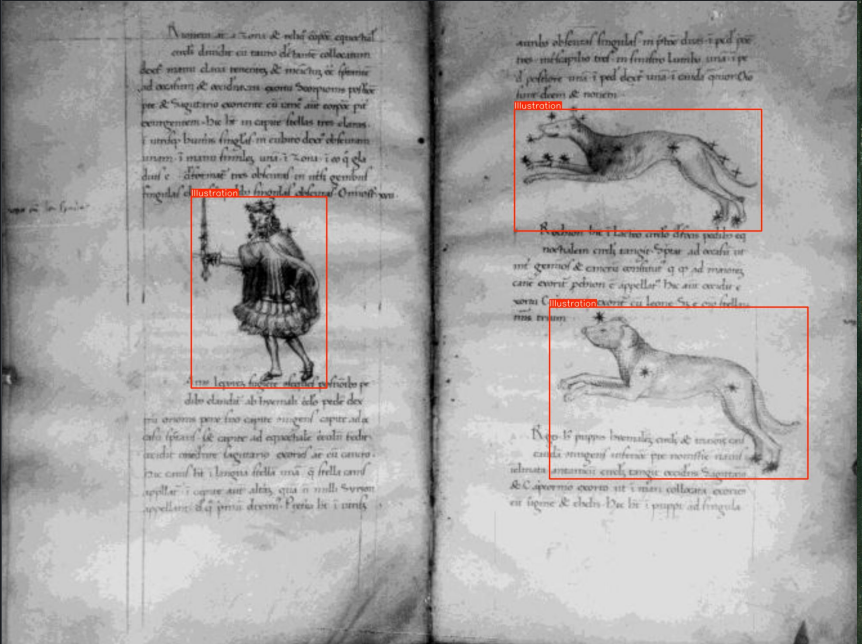
\includegraphics[scale=0.5]{img/aikon.png}
    \caption{Exemple de bounding boxes d'illustrations détectée sur Aikon au format Yolo}
    \label{fig:exemple-aikon}
    
\end{figure}

La particularité de ce format réside dans la normalisation des coordonnées. Les quatre valeurs géométriques ne sont pas exprimées en pixels absolus, mais en proportions relatives (des nombres flottants compris entre 0,0 et 1,0) calculées en fonction des dimensions totales de l'image. Les images d'un jeu de donnée au format yolo peut donc \^etre retravaillées sans avoir à modifier les annotations. 

Par exemple, une ligne d'annotation se présentera sous la forme : \texttt{3 0.18 0.89 0.29 0.18}. 


L'intérêt de ce format comparer à d'autres pour la constitution d'un corpus hétérogène comme GenHisDoc est qu'il permet de s'affranchir de la résolution original, qu'il s'agisse d'une image téléchargé à la résolution maximale d'une api IIIF ou un jeu de données beaucoup plus compressé et donc d'homogénéiser les données d'entrées avant la phase d'apprentissage. 

Certains corpus fournissent déjà une vérité terrain sous forme de boîtes englobantes (\textit{bounding boxes}), mais dans des formats incompatibles avec notre architecture. C'est le cas des formats historiques comme Pascal VOC ou de certains exports XML, qui utilisent des coordonnées absolues basées sur les pixels de l'image.

Généralement, ces formats classiques définissent une zone de deux manières :
\begin{itemize}
    \item Soit par les coordonnées du point supérieur gauche et du point inférieur droit : \texttt{\textbf{x\_min, y\_min, x\_max, y\_max}}
    
    \item Soit par les coordonnées du point supérieur gauche associées à la largeur et la hauteur absolues : \texttt{\textbf{x\_min, y\_min, w\_absolu, h\_absolu}}
\end{itemize}

Puisque le format YOLO exige des coordonnées relatives pointant depuis le centre de l'objet, une étape de conversion mathématique systématique est indispensable. Cette transformation nécessite de connaître les dimensions totales de l'image cible, à savoir sa largeur totale ($W$) et sa hauteur totale ($H$). 

Le passage des coordonnées absolues vers les valeurs normalisées exigées par YOLO s'opère grâce aux calcules suivants :

$$x_{YOLO} = \frac{x_{min} + x_{max}}{2 \times W}$$

$$y_{YOLO} = \frac{y_{min} + y_{max}}{2 \times H}$$

$$w_{YOLO} = \frac{x_{max} - x_{min}}{W}$$

$$h_{YOLO} = \frac{y_{max} - y_{min}}{H}$$

C'est ce calcul par ratio qui garantit au modèle une totale indépendance vis-à-vis de la résolution d'origine des numérisations.


\subsubsection{De la segmentation par pixels aux boîtes englobantes : le cas d'IlluHisDoc}

Plusieurs jeux de données comme IlluHisDoc et SynDoc (non utilisé dans notre travail) fournissaient à l'origine une vértié de terrain sous forme de masque de ségmentation où chaque pixel appartenant à une classe est coloré sur un fond noir. Il a fallu mettre en place un autre pipeline d'extraction géométrique. En utilisant la libraire \textit{Open Computer Vision} en Python, nous avons pu déduire les points extr\^emes des masques\footnote{Jules Musquin, scripte Réconciliation IlluHisDoc sur \href{https://github.com/Anarchiviste/GenHisDoc_Lab/blob/main/01_code/reconciliation_illuhisdoc.py}{Github}} (pixel le plus haut, le plus bas, le plus à gauche et le plus à droite pour chaque forme). À partir de ces limites absolues, nous avons pu retracer les bo\^ites englobantes avec des coordonés abolues et enfin appliqué la méthodologie décrite juste avant pour récupérer des coordonées normalisées au format YOLO. 

\begin{figure}[h]
        \centering
        \begin{subfigure}{0.48\textwidth}
            \centering
            
\includegraphics[scale=0.118]{img/btv1b10532593m_f14_seg.png}
        \end{subfigure}
        \hfill
        \begin{subfigure}{0.48\textwidth}
            \centering
            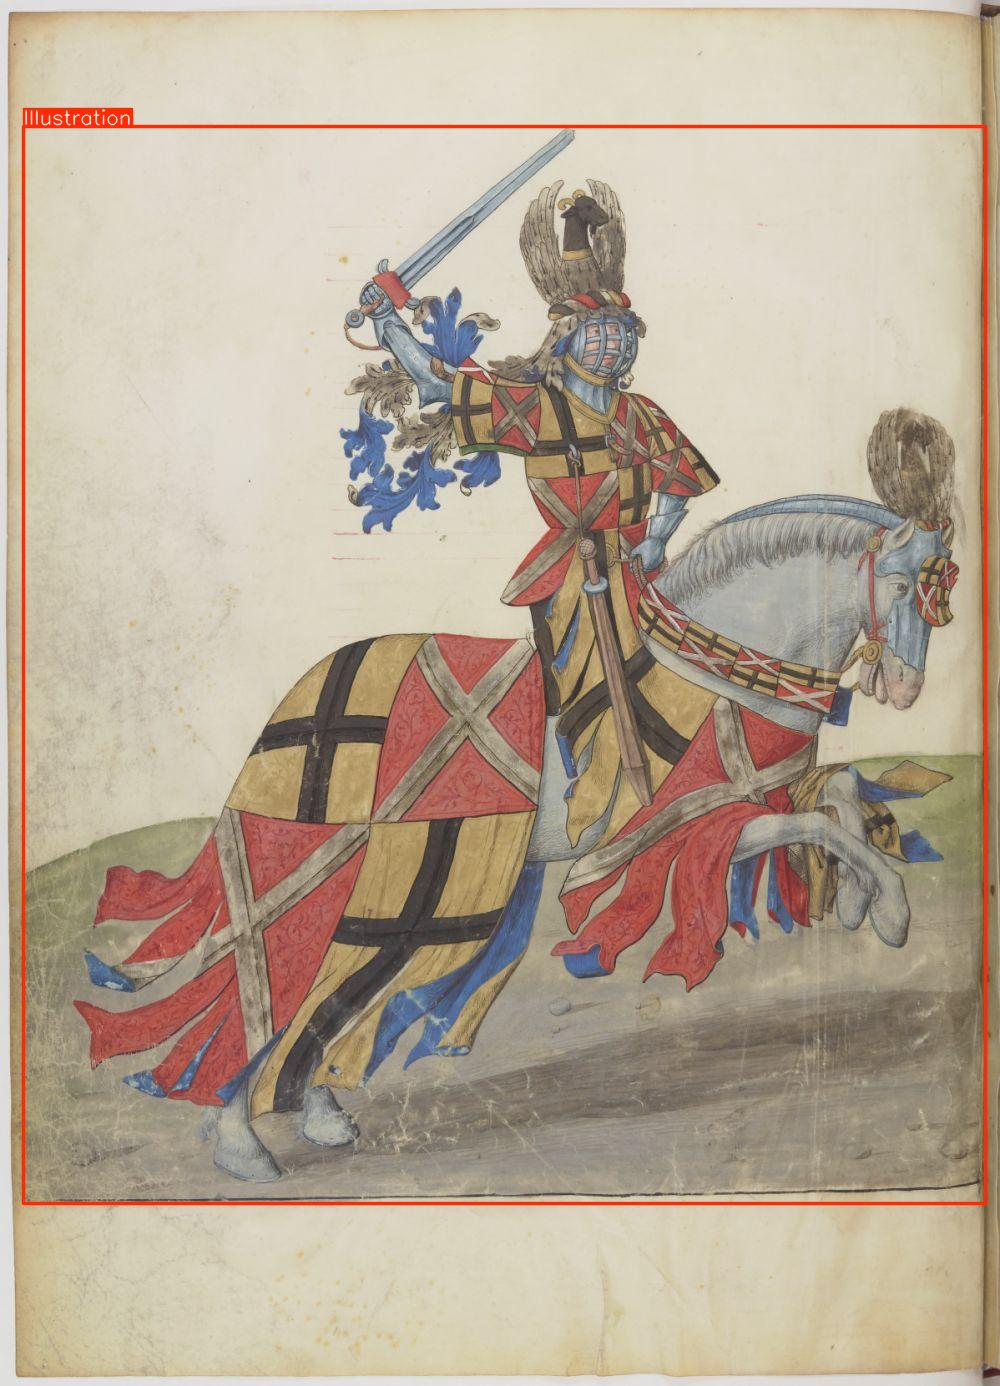
\includegraphics[scale=0.118]{img/illuhisdoc.jpg}
        \end{subfigure}
        \caption{Exemple d'une page et de son annotation en segmentation par pixel tiré du datatset IlluHisDoc.}
        \label{fig:segexemple}
\end{figure}

La complexité d'un conversion d'un dataset segmenté vient principalement de l'organisation interne des annotations. Par exemple \textit{IlluHisDoc } possède quatre classes d'annotations, mais l'organisation interne du dataset avec un dossier par classe d'annotation fait que la conversion vers des boites englobantes est relativement aisé comparé à un autre jeu de données comme \textit{SynDoc} ou chaque page peut avoir plusieurs instances segmentées de plusieurs classes différentes. La conversion d'un jeu de donnnées segmenté vers un jeu de données en boite englobante demande une réflexion sur la manière dont est construite l'annotation de segmentation au cas par cas. 

\subsection{Corriger des données}

Une fois toutes les annotations normalisées dans une ontologie et un format lisible commun, nous nous sommes concentré sur la tache de correction et d'enrichissement des données de GenHisDoc. C'est le moment où nous avons également d\^u intégrer un outil clef en main pour gérer les collections des documents à réannoter (des paquets de 1000 images et annotations), avoir un environnement graphique de travail (trancer les bo\^ites englobantes, les corriger, utiliser des fonctions de zoom, enregistrer les modifications), et également pouvoir exporter les annotations corrigées. Pour cela nous avons choisi d'utiliser la version gratuite de l'application \textit{Label Studio}.  

\subsubsection{L'environnement technique de correction : Label Studio}

\textit{Label Studio} est une application d'annotation de données développée par l'entreprise \textit{HumanSignal} et mis à disposition gratuitement en open-source dans une version limitée. L'application étant multimodale, elle possède son propre format d'annotation interne : le \textit{JSON Task}. 

\begin{figure}[h]
    \centering
    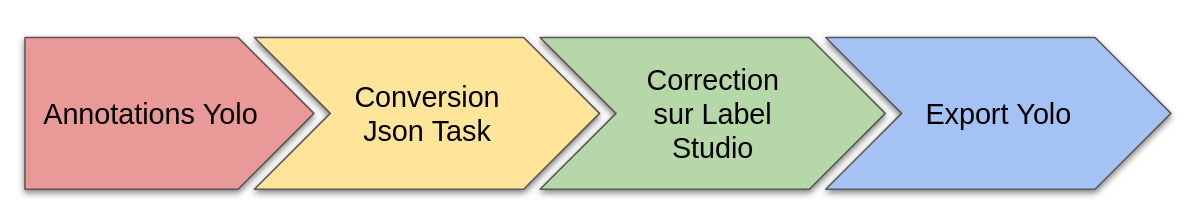
\includegraphics[scale=0.5]{img/LabelsStudio.png}
    \caption{Pipeline des tâches et conversion de format pour l'utilisation de Label Studio}
    \label{fig:LabelStudio}
\end{figure}

Label Studio prend \og techniquement \fg~en charge la conversion automatique du format YOLO vers le JSON Task ; cependant, la documentation mise à disposition est difficile d'utilisation et ignore certaines étapes intermédiaires pour pouvoir importer un projet\footnote{Label Studio Guide, \og Tutorial: Importing Local YOLO Pre-Annotated Images to Label Studio \fg, URL : \href{https://labelstud.io/blog/tutorial-importing-local-yolo-pre-annotated-images-to-label-studio/}{lien vers le blog}}. Nous avons donc réécrit et complété le tutoriel pour simplifier le travail de l'équipe qui voudrait réintégrer et corriger GenHisDoc à leurs travaux\footnote{Jules Musquin, \og Label Studio Reannotation \fg, dans \textit{GenHisDoc\_Lab} sur \href{https://github.com/Anarchiviste/GenHisDoc_Lab/blob/main/labelstudio_reannotation.md}{GitHub}}.

L'un des avantages de Label Studio tient par sa capacité à proposer un environnement applicatif modulaire pour les t\^aches d'annotations qui utilise un pseudo-langage pour sa mise en place. Cela permet de donner un bloc de code à copier-coller de la documentation aux paramètres de la tache d'annotation pour importer toute l'interface et l'ontologie à utiliser. 

\subsubsection{Corriger des annotations}

\begin{figure}[htbp]
\centering
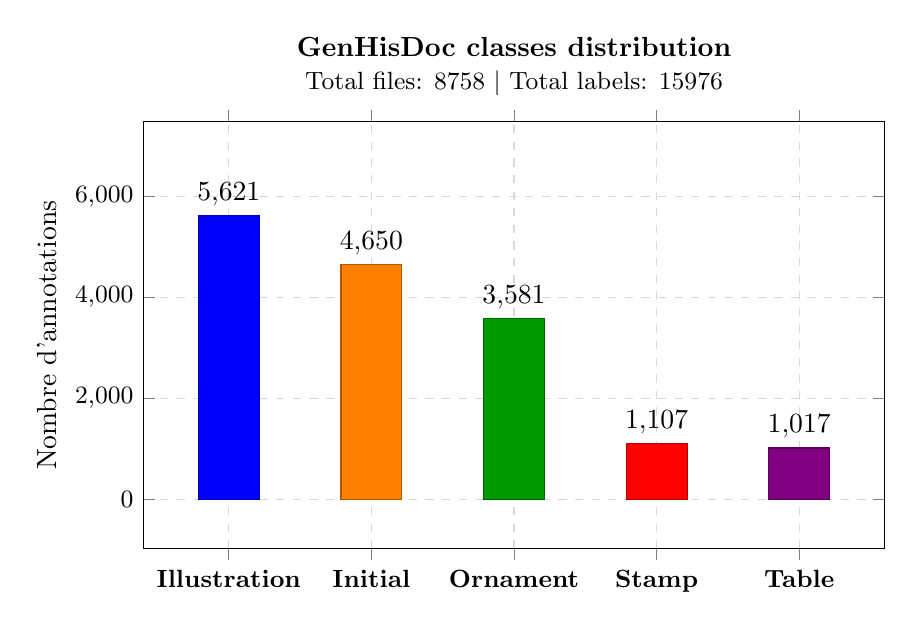
\begin{tikzpicture}
\begin{axis}[
    ybar,
    enlargelimits=0.15,
    ylabel={Nombre d'annotations},
    symbolic x coords={Illustration, Initial, Ornament, Stamp, Table},
    xtick={Illustration, Initial, Ornament, Stamp, Table},
    nodes near coords, % Affiche les valeurs au-dessus des barres
    nodes near coords align={vertical},
    x tick label style={rotate=0, anchor=north, font=\small\bfseries},
    y tick label style={font=\small},
    ymin=0, ymax=6500,
    bar width=22pt,
    height=7cm,
    width=11cm,
    grid=major,
    grid style={dashed, gray!30},
    title={\textbf{GenHisDoc classes distribution} \\ {\small Total files: 8758 $|$ Total labels: 15976}},
    title style={align=center}
]

\addplot[fill=blue, draw=blue!70!black, bar shift=0pt] coordinates {(Illustration, 5621)};
\addplot[fill=orange, draw=orange!70!black, bar shift=0pt] coordinates {(Initial, 4650)};
\addplot[fill=green!60!black, draw=green!40!black, bar shift=0pt] coordinates {(Ornament, 3581)};
\addplot[fill=red, draw=red!70!black, bar shift=0pt] coordinates {(Stamp, 1107)};
\addplot[fill=violet, draw=violet!70!black, bar shift=0pt] coordinates {(Table, 1017)};

\end{axis}
\end{tikzpicture}
\caption{Distribution des annotations par classe dans le dataset GenHisDoc.}
\label{fig:GenHisDocDistribution}
\end{figure}

La tache de correction des annotations présente plusieurs cas de figure plus ou moins long à prendre en compte lors de la présentation de la tache aux annotateur\pmm ices.

\begin{description}
    \item[La correction géométrique :] Un modèle de détection dans Aikon a correctement identifié la présence d'une illustration. Cependant, la boîte englobante est mal tracée et demande à être réajustée. 

    \item[La correction ontologique :] Dans S-VED, les \textit{Illustration} et les \textit{Printer's Mark} étaient annotées de manière séparées. Il faut donc que le correcteur réassigne le bon label à des boîtes englobantes déjà correctement tracées. 

    \item[L'ajout d'annotations manquantes (faux négatifs) :] Les modèles automatiques ou les corpus d'origine oublient fréquemment certains objets visuels (par exemple des lettrines de petite taille ou des éléments marginaux). L'annotateur doit alors tracer manuellement les boîtes englobantes absentes de la vérité terrain initiale.

    Certains jeux de données possèdent également des images avec des éléments qui nous intéressent (pour nous essentiellement les tables) sans les annoter. L'annotateur doit donc enrichir une annotation en rajoutant les éléments qui ne faisaient pas parti de l'ontologie du jeu de données d'origine. 

    \item[La suppression des prédictions erronées (faux positifs) :] Les algorithmes détectent parfois du bruit, des taches d'encre ou des artefacts de numérisation qu'ils interprètent à tort comme des zones d'intérêt. Ces boîtes invalides doivent être retirées du jeu de données.

    \item[Le découpage ou la fusion de zones complexes :] Dans certains cas d'enluminures ou d'ornements imbriqués, l'outil initial a regroupé plusieurs éléments distincts au sein d'une unique grande boîte, ou au contraire a morcelé une illustration continue. Le correcteur doit scinder ou fusionner ces zones pour respecter les granularités fixées par l'ontologie GenHisDoc. C'est de loin la t\^ache de correction la plus longue et éprouvante. 
\end{description}